\documentclass[tikz,border=3pt]{standalone}
\usepackage[utf8]{inputenc}
\usepackage[T1]{fontenc}
\usepackage{lmodern}
\renewcommand{\familydefault}{\sfdefault}
\usepackage{sansmath}\sansmath
\usepackage{chemfig}
\usepackage{pgfplots}\pgfplotsset{compat=1.18,/pgf/number format/use comma,/pgf/number format/1000 sep={.}}
\usetikzlibrary{arrows.meta,calc,positioning,decorations.pathmorphing,patterns}
% paleta del sitio
\definecolor{nar}{HTML}{E8680C}\definecolor{narc}{HTML}{FFB35C}\definecolor{hielo}{HTML}{FFF3E8}
\definecolor{tinta}{HTML}{1D1D1F}\definecolor{gris}{HTML}{6E6E73}\definecolor{lila}{HTML}{7C5CF0}
\definecolor{azul}{HTML}{2F6FD6}\definecolor{menta}{HTML}{17A673}\definecolor{coral}{HTML}{E8342A}
\begin{document}
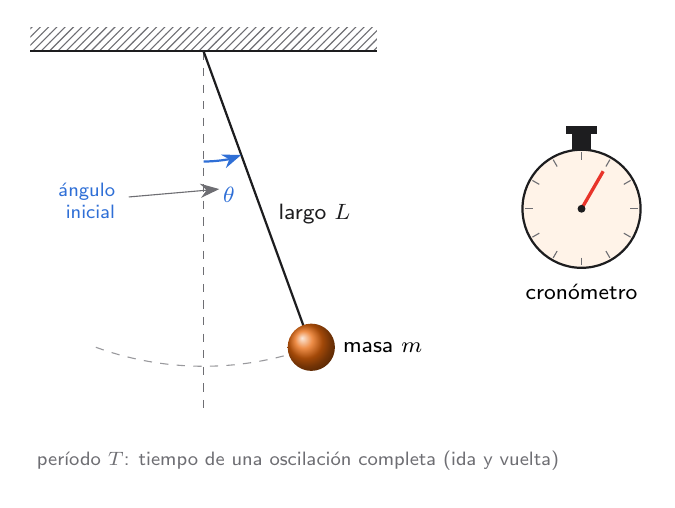
\begin{tikzpicture}[font=\footnotesize,>={Stealth[length=2.4mm]}]
\fill[pattern=north east lines,pattern color=gris] (-2.2,0) rectangle (2.2,0.3);
\draw[thick,tinta] (-2.2,0) -- (2.2,0);
\coordinate (O) at (0,0);
\draw[dashed,gris] (O) -- (0,-4.6);
\draw[dashed,gris!70] (-110:4) arc (-110:-70:4);
\coordinate (B) at (-70:4);
\draw[thick,tinta] (O) -- (B) node[pos=0.55,right=2pt,text=tinta] {largo $L$};
\shade[ball color=nar] (B) circle (0.3);
\node[right=8pt] at (B) {masa $m$};
\draw[->,azul,thick] (-90:1.4) arc (-90:-70:1.4);
\node[azul] at (-80:1.85) {$\theta$};
\node[azul,align=right,anchor=east,font=\scriptsize] at (-1.0,-1.9) {ángulo\\inicial};
\draw[->,gris] (-0.95,-1.85) -- (0.2,-1.75);
% cronómetro
\begin{scope}[shift={(4.8,-2.0)}]
\draw[thick,tinta,fill=hielo] (0,0) circle (0.75);
\fill[tinta] (-0.12,0.75) rectangle (0.12,0.95);
\fill[tinta] (-0.2,0.95) rectangle (0.2,1.05);
\foreach \a in {0,30,...,330} \draw[gris] (\a:0.62) -- (\a:0.72);
\draw[very thick,coral] (0,0) -- (60:0.55);
\fill[tinta] (0,0) circle (0.05);
\node at (0,-1.05) {cronómetro};
\end{scope}
\node[align=center,text=gris,font=\scriptsize] at (1.2,-5.2) {período $T$: tiempo de una oscilación completa (ida y vuelta)};
\end{tikzpicture}
\end{document}
